% The figure eight with its two generating loops a and b.
% Source: book/tex/topology/fundamental-group.tex (§ Fundamental groups).
\documentclass[border=2mm]{standalone}
\usepackage{tikz}
\usetikzlibrary{arrows.meta,decorations.markings}
\tikzset{loparr/.style={decoration={markings,
  mark=at position 0.5 with {\arrow{Latex}}},postaction={decorate}}}
\begin{document}
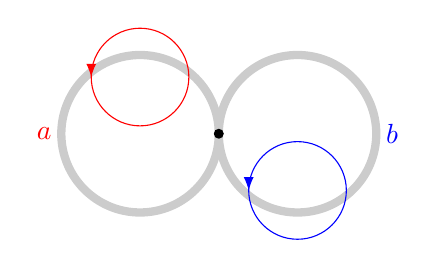
\begin{tikzpicture}[scale=1]
  \draw[gray!40,line width=3pt] (-1,0) circle (1);
  \draw[gray!40,line width=3pt] (1,0) circle (1);
  \fill (0,0) circle (1.8pt);
  \draw[red,loparr] (-1,0.72) circle (0.62);
  \draw[blue,loparr] (1,-0.72) circle (0.62);
  \node[red,left] at (-2,0) {$a$};
  \node[blue,right] at (2,0) {$b$};
\end{tikzpicture}
\end{document}
